
\hypertarget{Le-travail-a-distance}{%}
\chapter{Le travail à distance}\label{Le-travail-a-distance}}

Dans cette partie nous verrons dans un premier temps les méthodes qui nous on permis de pouvoir continuer a travailler à distance. Puis dans un second temps nous verrons les outils que nous avons utilisé pour celà ainsi que leur interet. A savoir GitHub pour le stockage des programmes et de la documentation. Puis collab qui nous grâce auquel nous avons pu coder en ligne. Et logiquement on enchainera avec tensorflow qui fonctionne particuliérement bien avec colab. Puis on finira avec LaTex qui a été l'un de mes principaux outils de travail.

\hypertarget{Organisation-du-travail-a-distance}{%}
\section{Organisation du travail à distance}\label{Organisation-du-travail-a-distance}}


Comme vous le savez certainement durant cette année 2020 nous avons été touché par la crise du coronavirus qui nous à conduit à être confinés nous forçant à travailler uniquement à distance.

Ces circonstances très particuliéres ont grandement affecté notre travail particulérement au début où nous avons dû régler de nombreux problémes techniques et organisationels. Cependant en nous forçant à nous adapter à ces nouvelles conditions, cette crise nous a permis de grandement augmenter nos competances en "télétravail".

Ainsi malgré des débuts léthargiques nous avons mis en place une "routine de travail" qui était la suivante :
\begin{itemize}
\item Des visio-conférences quotidiennes nous permettant d'organiser et de synchroniser notre travail
\item Un groupe whatsap dédié à mon stage afin de communiquer le plus efficacement possible
\item Un Github privé dédié afin de partager l'ensemble du projet
\item Un partage régulier de google collab via google drive
\end{itemize}

\hypertarget{Outils-utilisuxe9s}
\subsection{Présentation de GitHub}
\label{Pruxe9sentation-de-GitHub}}

\begin{figure}[h]
  \begin{center}
  
\includegraphics[width=5cm]{./images/github.jpg}
  \end{center}
\end{figure}

Nous pouvons définir GitHub comme une plateforme de développement de projet in formatique en groupe. Elle s'implifie grandement le développement de projets. Elle permet de versioner ses programme et d'y apporter des modification en temps réel à plusieurs.

\hypertarget{Pourquoi-Github}{%}
\subsubsection{Pourquoi Github}
\label{Pourquoi-Github}}
Car celà permet une certaine synergie avec nos autres outils que nous verrons plus tard. Cette plateforme permet une facilité de développement de par sa fonctionnalité de versionnage de notre code à chaque changement ce qui permet une mise à jour dynamique ainsi qu'une relative facilité à retourner à un état antérieur de notre programme ce qui permet une facilité de débogage.Nous pouvons d'ailleurs dire que ce rappport est entreposer sur Github et qu'il peut-être récupérer facilement.Cette plateforme est aussi très connue dans le monde de la programmation ce qui sera utile pour notre futur professionnel.

\hypertarget{Pruxe9sentation-de-Google-Colab}{%}
\subsection{Présentation de Google Colab}
\label{Pruxe9sentation-de-Google-Colab}}

\begin{figure}[h]
\begin{center}

\includegraphics[width=5cm]{./images/Colab_logo.png}
\end{center}
\end{figure}

Colab peut-être défini comme étant une plateforme d'éxécution pour notre code
il permet du fait que ce soit la puissance de calcul d'ordinateur géré par Google une vitesse d'exécution ainsi qu'une vitesse de téléchargement de base de données supérieure à celle qui nous est disponible en local.

\hypertarget{Pourquoi-Colab}{%}
\subsubsection{Pourquoi Colab}
\label{Pourquoi-Colab}}
En premier lieu pour faciliter l'exécution du code car elle ne se fais pas en local ce qui permet une exécution quasi immédiate du code sans aucune installation. Il est aussi facile de mettre sur github du code produit avec colab car ces deux plateformes sont liées. Il permet de par l'utilisation du format Jupyter notebook de mélanger code et texte (peu aussi comporter des images) dans notre notebook.

Voilà un exmple d'exécution avec colab:

\begin{figure}[h]
\begin{center}
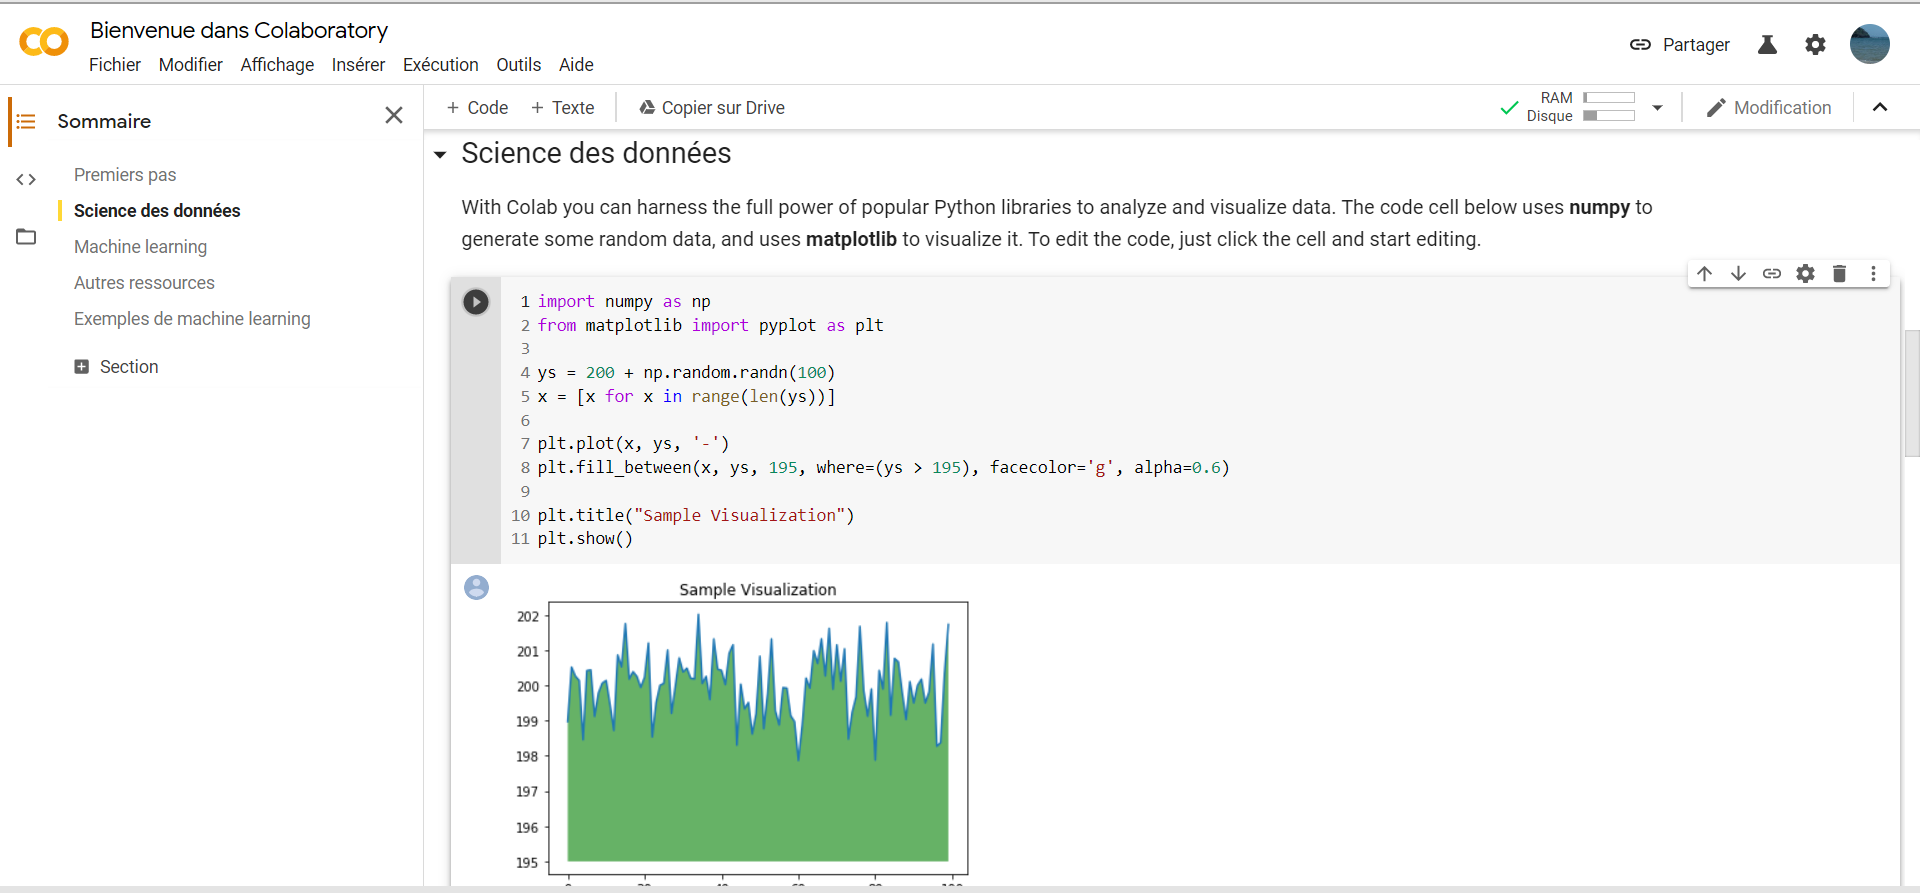
\includegraphics[width=15cm]{./images/Cap_colab.PNG}
\caption{Nous avons ici un exemple de code exécuté avec colab.}
\end{center}
\end{figure}

\hypertarget{Tensorflow}{%
\subsection{TensorFlow}%
\label{Tensorflow}}


\begin{center}
\label{fig:Tensorflow_logo}
\centering

\includegraphics[width=5cm]{./images/Tensorflow_logo.png}
\begin{figure}[h!]
\caption{Logo de Tensorflow}
\end{figure}
\end{center}


TensorFlow est un framework open source,
multiplateforme d'apprentissage automatique développée par Google Brain,
en C++ avec une interface pour Python.
Sa premiere version est publiée par Google le 9 novembre 2015.
L'intérêt de ce framework est de limiter les coûts de développement des solutions à base
de réseaux de neurones, en réunissant des fonctionnalités permettant,
en quelques lignes de code de construire des réseaux complexes.
Tensorflow permet donc de simplifier beaucoup de choses dans
le domaine de l'apprentissage automatique.
Son autre intérêt est de fournir des interfaces pour pouvoir exécuter les calculs sur
des accélérateurs graphiques et surtout de les prendre en charge
de façon complétement transparente pour les utilisateurs.
Les gains de vitesse peuvent atteindre ainsi un facteur 10 quand le même modèle est exécuté
sur une carte graphique.

Le concurrent principal de TensorFlow est pyTorch, utilisé par FaceBook.

\hypertarget{Pruxe9sentation-de-LaTex}{%}
\subsection{Présentation de LaTex}
\label{Pruxe9sentation-de-LaTex}}

\begin{figure}[h]
  \begin{center}

\includegraphics[width=5cm]{./images/Latex.png}
\end{center}
\end{figure}

Nous pouvons dire que LaTex est un langage de traitement de texte tel que le markdown qui permet de mettre en forme notre texte de manière \"scientifique\" cela veut dire que. LaTex permet une facilité d'écriture des équations et de toutes les écritures mathématiques. Ce langage permet de par ses nombreux packages une quasi-infinité de possibilités. Il permet également de générer des fichiers pdf facilement et de manière automatique. Raison qui m'as logiquement poussé à choisir ce langage afin de générer mes pdf.
